In this section, we present the strategies and tools used to implement the heuristics mentioned in the previous section.
\subsection{Call-Graph Analysis}
To profile the android application, we used the T.J Watson Libraries for Analysis (WALA)~\cite{wala} which provides static analysis
of Java bytecode. WALA provides an API to the developer using which the application can be analyzed and a Call Graph can be
constructed. A call graph is a directed graph that can be used to identify relationships between method calls in a program.
Call graphs can be constructed either statically or dynamically, we use a static approach for our analysis. A static
call graph cannot represent the exact execution flow of the program and hence it is usually an over-approximation of
the actual dynamic execution. Static call graphs can be constructed with various degrees of precision as studied by
~\cite{cgbuild}. A precise call graph should be context-sensitive and include information about the different paths through which
each procedure can be invoked. The call graph construction algorithms differ based on the number of sets that are used to find the
run-time values of the expressions. WALA profiler can construct a call graph using Rapid Type Analysis (RTA) or a Control-Flow-Analysis
(k-CFA). The RTA approach uses one set for the whole program and scales well for applications with a large code-base. k-CFA uses
several sets per expression and provide higher precision about the program flow.
We used the WALA profiler to produce the RTA and the 0-CFA based call graph. For large applications, the CFA algorithm took a long time to
compute the call graph and resolve all dependencies. Hence, we perform all our static analysis using the RTA builder. Using the WALA API,
we wrote a profiler which identifies native methods and their corresponding parent in the application.
This information is used for estimating the time difference between the Parent and next Native for calculation of the Parent-to-Native Execution
Time heuristic.

Figure ~\ref{fig:native_total} shows the percentage of native methods present in the benchmarks and the applications we used for our analysis.
The percentage ranges from around 6% to 10%. We observed that this percentage doesn't drastically vary the performance of COMET since there
are usually certain specific native method calls that force the offloaded thread on the server to abort and migrate it back to the client. For instance, nativeConfig
and nativeSetPixels in the photoshop application, nativeConfig in fractal always made the thread execution abort on the server. Since these native methods set the unsafe point, sometimes COMET misses the opportunity to migrate non-native code while waiting to cross the threshold limit. Therefore, these methods helped us target the next non-native code with significant amount of computation for migration. 

The information generate by the WALA profiler was coupled with a dynamic profiling technique to identify the methods of interest.
We used the Dalvik Debugger Monitor Service (DDMS) tool to get the execution times of all the methods in the application. DDMS can perform
thread level profiling by attaching to the process that we wish to debug. DDMS has information about all the processes running on the device
that it is connected to. Every process runs in its own virtual machine (VM). Once DDMS retrieves the process ID (PID) via adb, it opens a
connection to the VM's debugger and can now communicate with the VM. All the process activity is forwarded to the debugger from the process VM
and is captured by DDMS. DDMS produces a trace log file of the profiled process. To view this log file in readable form, we used the
$dmtracedump$ tool. The output of this tool depicts the call-stack of the program execution along with individual method execution times.

To extract relevant information from the DDMS log file, we used the output generated by the WALA profiler to find the native methods' and their
parent methods' execution time. The log file and the WALA ouput were fed to a python script that printed the execution times of all the
necessary methods. Another script was used to find the Parent-to-Native execution time.

%-------------------------------------------------------%
\begin{figure} [thf*]
\centering
\begin{tabular}{c}
\begin{minipage}[b]{0.5\textwidth}
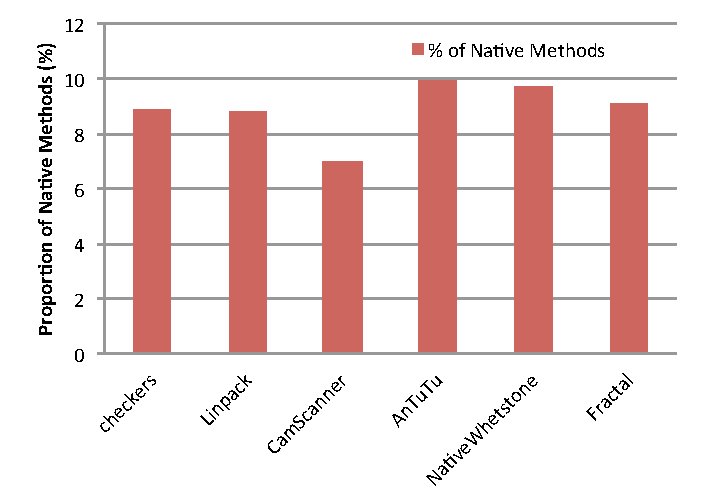
\includegraphics[width=0.95\textwidth]{figs/native_total.pdf}
\end{minipage}
\end{tabular}
\caption{Results from the Wala profiler with the proportion of native methods per application}
\label{fig:native_total}
\end{figure}

\subsection{Bandwidth Limitation}
As stated in Section~\ref{sec:back} we wanted to include the bandwidth in our scheduling decision making logic. To make the current bandwidth conditions avaialble to the device, we ran a daemon similar in nature to the \texttt{tcpmux} daemon used in COMET. The \texttt{tcpmux} daemon helps in communication between the client and server and also in providing the latest RTT values to the decision engine. When the decision engine is invoked for the first time, the engine connects to the \texttt{tcpmux} daemon running locally using \texttt{connect} and gets the latest RTT value. This RTT value is obtained only once during the lifetime of the thread. We implemented a similar daemon that would provide for the latest bandwidth conditions. The bandwidth daemon internally ran the \texttt{iperf} tool to estimate the bandwidth. The daemon was configured to recalculate the bandwidth periodically after every 10 seconds.

To limit the bandwidth available to the device, we explored two options - \texttt{dummynet} and \texttt{tc}. Owing to certain kernel module incompatabilities with \texttt{dummynet}, we used \texttt{tc} to limit the bandwidth for our experiments. \texttt{tc} is not available immediately in production devices and we had to rebuild the kernel to provide support for \texttt{tc}. After tc was eanbled in the kernel, we used the Hierarchical Token Bucket (HTB) queuing discipline to limit both the upload and download bandwidth. We used a shell script to dynamically change the bandwidth over different executions of the application.

Studying the code, we observed that the data to be transferred is collected much after a decision has been made to migrate it. Thus, the data size to be transferred is available just before a \texttt{write} call to the socket. We implemented our decision logic at this stage in the application's execution. We query the bandwidth daemon to get the latest avaialble bandwidth. Next, we compare the size of data to be transferred to a threshold derived from the latest bandwidth and then take a final decision whether to offload the thread or not.

The results of incorporating the network bandwidth are presented in Section~\ref{sec:results}. Adding this check did not lead to any performance improvement
over the baseline heuristic used in COMET.
